\section{Experiments}

\subsection{Setup}

\noindent\textbf{Dataset.} COD10K-v3~\cite{fan2020cod10k}: 3,040 camouflaged training images, 2,026 camouflaged test images across 78 categories (aquatic, terrestrial, flying, amphibian).

\noindent\textbf{Implementation.} SAM ViT-H backbone. Training images augmented with horizontal flips (6,080 total). Decoder training: $\sim$90 min on A100 with pre-computed embeddings. LLPM+decoder training: $\sim$7.5 hrs (live encoder pass). Decoder checkpoint: 16MB.

\subsection{Main Results}

\Cref{tab:main} presents results across all prompt strategies.

\begin{table*}[t]
\centering
\caption{\textbf{Main results} on COD10K camouflaged test set (2,026 images). Best per-column in \textbf{bold}. Decoder-only fine-tuning improves all metrics across all prompt types; LLPM adds further gains on edge prompts.}
\label{tab:main}
\small
\begin{tabular}{llccccccc}
\toprule
Model & Prompt Strategy & mIoU & Dice & $S_\alpha$ & $E_\phi$ & $F_\beta^w$ & MAE$\downarrow$ & Bnd.~F1 \\
\midrule
Base SAM & Center-of-Mass (1pt) & 0.572 & 0.654 & 0.743 & 0.830 & 0.706 & 0.068 & 0.502 \\
Base SAM & Edge (1pt) & 0.205 & 0.251 & 0.481 & 0.597 & 0.241 & 0.163 & 0.281 \\
Base SAM & Multi-Pt Grid (4pt) & 0.682 & 0.761 & 0.812 & 0.897 & 0.802 & 0.046 & 0.600 \\
Base SAM & Multi-Pt Random (3pt) & 0.727 & 0.814 & 0.830 & 0.929 & 0.831 & 0.043 & 0.648 \\
\midrule
Decoder-only & Center-of-Mass (1pt) & 0.738 & 0.819 & 0.847 & 0.942 & 0.819 & 0.028 & 0.702 \\
Decoder-only & Edge (1pt) & 0.694 & 0.779 & 0.810 & 0.922 & 0.750 & 0.034 & 0.666 \\
Decoder-only & Multi-Pt Grid (4pt) & \textbf{0.756} & \textbf{0.835} & \textbf{0.861} & \textbf{0.951} & \textbf{0.841} & \textbf{0.024} & \textbf{0.720} \\
Decoder-only & Multi-Pt Random (3pt) & \textbf{0.776} & \textbf{0.855} & \textbf{0.874} & \textbf{0.960} & \textbf{0.863} & \textbf{0.021} & \textbf{0.739} \\
\midrule
LLPM + Decoder & Center-of-Mass (1pt) & \textbf{0.740} & \textbf{0.820} & \textbf{0.847} & \textbf{0.938} & \textbf{0.820} & \textbf{0.028} & \textbf{0.706} \\
LLPM + Decoder & Edge (1pt) & \textbf{0.719} & \textbf{0.802} & \textbf{0.827} & \textbf{0.933} & \textbf{0.778} & \textbf{0.029} & \textbf{0.691} \\
LLPM + Decoder & Multi-Pt Grid (4pt) & 0.755 & 0.833 & 0.856 & 0.946 & 0.833 & 0.025 & 0.721 \\
LLPM + Decoder & Multi-Pt Random (3pt) & 0.770 & 0.850 & 0.865 & 0.954 & 0.847 & 0.022 & 0.734 \\
\bottomrule
\end{tabular}
\end{table*}

Decoder-only fine-tuning improves mIoU on all four prompt types by +4.9 to +48.9 absolute points. The LLPM adds +2.6 mIoU on edge prompts, where boundary disambiguation matters most.

\subsection{Prompt Robustness}

\begin{table}[t]
\centering
\caption{\textbf{Prompt robustness.} Base SAM is highly sensitive to prompt quality (mIoU 0.205--0.727); our decoder narrows this to 0.694--0.776.}
\label{tab:improvement}
\small
\begin{tabular}{lcccc}
\toprule
Prompt Type & Base & Ours & $\Delta$ & Rel.~$\Delta$ \\
\midrule
Center-of-Mass & 0.572 & 0.738 & +0.166 & +28.9\% \\
Edge (Single) & 0.205 & 0.694 & +0.489 & \textbf{+238.1\%} \\
Multi-Pt Grid & 0.682 & 0.756 & +0.074 & +10.9\% \\
Multi-Pt Random & 0.727 & 0.776 & +0.049 & +6.7\% \\
\bottomrule
\end{tabular}
\end{table}

Base SAM's mIoU varies 3.5$\times$ across prompt types (0.205 to 0.727); the specialized decoder varies only 1.1$\times$ (0.694 to 0.776). Edge prompts, where the click lands on the boundary between object and background, show the largest absolute gain (+48.9 mIoU), indicating that decoder fine-tuning learns to resolve boundary ambiguity rather than memorize prompt-mask associations.

\subsection{Per-Category Analysis}

\begin{table}[t]
\centering
\caption{\textbf{Per-category mIoU} (Center-of-Mass prompt). Terrestrial animals, the hardest category, show the largest relative gain.}
\label{tab:category}
\small
\begin{tabular}{lcccr}
\toprule
Category & $N$ & Base & Ours & Rel.~Gain \\
\midrule
Amphibian & 124 & 0.680 & 0.825 & +21.4\% \\
Aquatic & 474 & 0.563 & 0.720 & +27.9\% \\
Flying & 714 & 0.610 & 0.767 & +25.6\% \\
Terrestrial & 699 & 0.519 & 0.703 & \textbf{+35.5\%} \\
\bottomrule
\end{tabular}
\end{table}

Terrestrial animals (insects on bark, lizards on rocks) show the largest gain (+35.5\%), consistent with their strong background-matching camouflage. Aquatic animals follow at +27.9\%.

\subsection{Error Analysis}
\label{sec:error_analysis}

To understand \emph{where} our model still fails, we analyze the worst-performing images (bottom quartile by IoU) and categorize them using image metadata computed during evaluation.

\noindent\textbf{Failure categories.} We define five automatic categories:
\begin{itemize}
    \item \textbf{Dark}: image brightness $<$ 80 (out of 255)
    \item \textbf{Tiny}: foreground pixels $<$ 1\% of image area
    \item \textbf{Thin/elongated}: GT bounding box aspect ratio $>$ 5:1
    \item \textbf{Disjoint}: multiple connected components in GT mask
    \item \textbf{General}: none of the above
\end{itemize}

\begin{table}[t]
\centering
\caption{\textbf{Error analysis.} Mean IoU on the 400 worst-performing images, grouped by failure category. LLPM improves on all categories except the rare thin/elongated case ($N\!=\!2$).}
\label{tab:error_analysis}
\small
\begin{tabular}{lrccc}
\toprule
Category & $N$ & Base & Spec. & LLPM \\
\midrule
Disjoint & 175 & .213 & .303 & \textbf{.371} \\
Dark & 104 & .316 & .326 & \textbf{.366} \\
General & 65 & .352 & .342 & \textbf{.413} \\
Tiny & 54 & .289 & .261 & \textbf{.292} \\
Thin/elongated & 2 & .004 & \textbf{.346} & .222 \\
\bottomrule
\end{tabular}
\end{table}

\noindent\textbf{Findings.}
Failures are not random (\cref{tab:error_analysis}). Disjoint objects (multiple connected components, 44\% of failures) and dark images (26\%) dominate. The LLPM improves over the decoder-only model in all major categories: +6.8 mIoU on disjoint objects, +7.1 on the general bin, and +4.0 on dark images. These gains show that the LLPM's boundary-contrast amplification helps beyond edge prompts alone. Tiny objects ($<$1\% foreground pixels) remain the hardest category (mean IoU 0.29); scale-aware augmentation or multi-scale features are likely needed here.

\subsection{Comparison with Existing Methods}

\begin{table}[t]
\centering
\caption{\textbf{Comparison with COD methods} on COD10K test set. This table contextualizes decoder-only adaptation within the broader COD landscape. \emph{Important:} our method uses oracle GT-derived prompts, while dedicated methods are fully automatic; these are not head-to-head comparisons.\textsuperscript{$\dagger$}}
\label{tab:comparison}
\small
\resizebox{\columnwidth}{!}{%
\begin{tabular}{llcccc}
\toprule
Method & Venue & $S_\alpha$ & $E_\phi$ & $F_\beta^w$ & MAE$\downarrow$ \\
\midrule
\multicolumn{6}{l}{\textit{Fully automatic (no prompts)}} \\
SINet~\cite{fan2020cod10k} & CVPR'20 & .776 & .864 & .631 & .043 \\
PFNet~\cite{mei2021pfnet} & CVPR'21 & .800 & .877 & .660 & .040 \\
SINet-V2~\cite{fan2022sinetv2} & TPAMI'22 & .815 & .887 & .680 & .037 \\
SegMaR~\cite{jia2022segmar} & CVPR'22 & .833 & .899 & .724 & .034 \\
ZoomNet~\cite{pang2022zoomnet} & CVPR'22 & .838 & .911 & .729 & .029 \\
\midrule
\multicolumn{6}{l}{\textit{SAM-based (encoder/prompt tuning)}} \\
SAM-Adpt.~\cite{chen2023samadapter} & ICCVW'23 & .883 & .918 & .801 & .025 \\
COMPr.~\cite{hao2024comprompter} & SCIS'24 & \textbf{.889} & .949 & .821 & \textbf{.023} \\
\midrule
\multicolumn{6}{l}{\textit{Decoder-only (ours, oracle prompts\textsuperscript{$\dagger$})}} \\
\textbf{Ours} (Grid) & --- & .861 & .951 & .841 & .024 \\
\bottomrule
\end{tabular}}
\vspace{1pt}
{\footnotesize \textsuperscript{$\dagger$}Prompts derived from GT masks. In deployment, prompts come from users or upstream detectors; performance depends on prompt quality, not our adaptation.}
\end{table}

\Cref{tab:comparison} places decoder-only adaptation in the broader COD landscape. The comparison is contextual, not head-to-head: our method uses oracle GT-derived prompts, while dedicated COD methods are fully automatic. Under this protocol, decoder-only adaptation recovers strong performance with no new decoder parameters and 90-minute training, but does not surpass encoder-adaptation methods (SAM-Adapter, COMPrompter) on $S_\alpha$ or MAE. This gap is consistent with encoder and decoder specialization addressing different aspects of the problem.

\subsection{Cross-Dataset Generalization}

\begin{table}[t]
\centering
\caption{\textbf{Cross-dataset generalization} (Center-of-Mass prompt). Our decoder is trained only on COD10K and evaluated on held-out datasets without retraining.}
\label{tab:crossdataset}
\small
\begin{tabular}{llcccc}
\toprule
Dataset & Model & mIoU & $S_\alpha$ & $E_\phi$ & MAE$\downarrow$ \\
\midrule
\multirow{3}{*}{CAMO (250)} & Base SAM & .489 & .672 & .748 & .122 \\
 & Decoder-only & .658 & .787 & .875 & .075 \\
 & LLPM+Decoder & \textbf{.677} & \textbf{.797} & \textbf{.887} & \textbf{.073} \\
\midrule
\multirow{3}{*}{NC4K (4{,}121)} & Base SAM & .567 & .728 & .805 & .093 \\
 & Decoder-only & .741 & .841 & .924 & .048 \\
 & LLPM+Decoder & \textbf{.752} & \textbf{.848} & \textbf{.929} & \textbf{.045} \\
\bottomrule
\end{tabular}
\end{table}

The decoder is trained only on COD10K. On CAMO, mIoU improves from 0.489 to 0.677 (+18.8 points); on NC4K (4,121 images), from 0.567 to 0.752 (+18.5 points). The LLPM's additional gain also replicates on both datasets without retraining, suggesting that the decoder learns camouflage-general cues rather than COD10K-specific patterns.

\subsection{Generalization to Regular Images}

\begin{figure}[t]
\centering
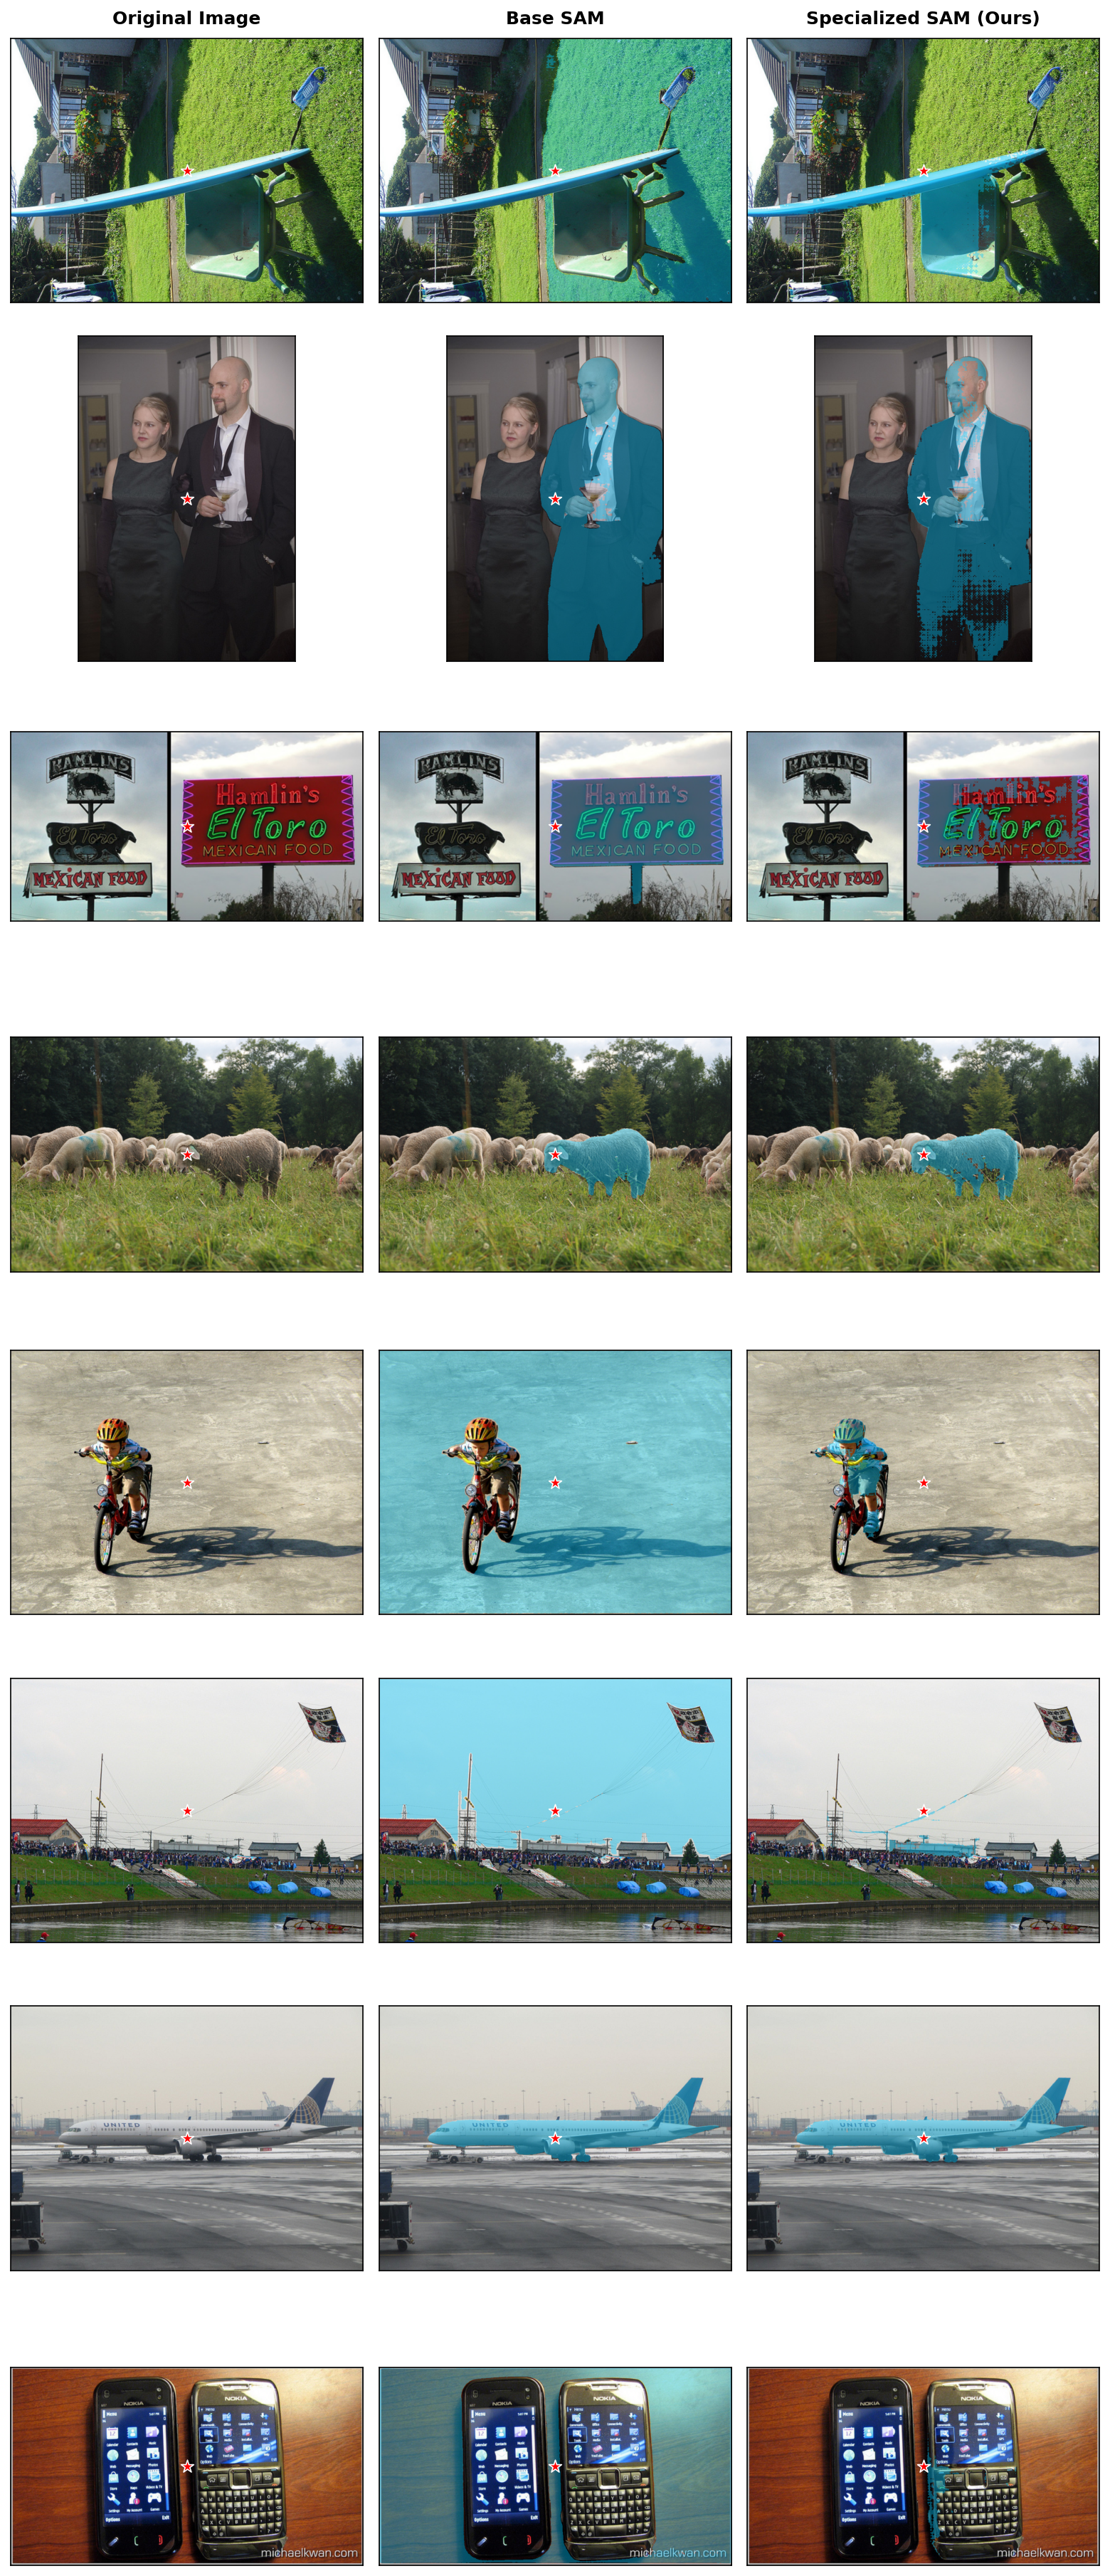
\includegraphics[width=\columnwidth]{figures/coco_comparison.png}
\caption{\textbf{Qualitative results on regular COCO images} (fixed image-center prompt, no ground truth used). As a sanity check, camouflage specialization does not appear to cause obvious degradation on regular images: our decoder often produces tighter masks. Base SAM over-segments in several cases (rows 3 and 6), while our decoder remains conservative.}
\label{fig:coco}
\end{figure}

A reasonable concern is whether camouflage specialization degrades performance on ordinary images. \Cref{fig:coco} gives a qualitative check on random COCO val2017 images using a fixed image-center prompt (no ground truth). The specialized decoder does not obviously degrade on these scenes. In several cases it produces \emph{tighter} masks than base SAM, which over-segments background when the center prompt is ambiguous. Quantitative evaluation on general images is left for future work.
